\documentclass[a4paper,10pt]{article}
\usepackage[margin=1.4in]{geometry}
\usepackage[swedish]{babel}
\usepackage[utf8]{inputenc}
\usepackage{titlesec}
\usepackage{titling}
\usepackage{todonotes}



\setlength{\parskip}{1em}
\setlength{\parindent}{0pt}
\titlespacing{\section}{0pt}{\parskip}{-\parskip}
\titlespacing{\subsection}{0pt}{\parskip}{-\parskip}
\titlespacing{\subsubsection}{0pt}{\parskip}{-\parskip}
\titlespacing{\part}{0pt}{\parskip}{-\parskip}

\def\ftitle{Statusrapport Iteration 2}
\def\fversion{1.0}

\begin{document}

\begin{titlepage} % Suppresses displaying the page number on the title page and the subsequent page counts as page 1
	\newcommand{\HRule}{\rule{\linewidth}{0.5mm}} % Defines a new command for horizontal lines, change thickness here

	\center % Centre everything on the page

	%------------------------------------------------
	%	Headings
	%------------------------------------------------

	\textsc{\LARGE Linköpings universitet \\ \vspace{0.2em} Institutionen för datavetenskap }\\[2cm]

    \large\today

    \vspace{1cm}


	%------------------------------------------------
	%	Title
	%------------------------------------------------

	\HRule\\[0.4cm]

	{\huge\bfseries Schemaläggningsstöd för  kirurgi \vspace{.1em} \\ \ftitle }\\[0.4cm] % Title of your document

	\HRule\\[1cm]

	%------------------------------------------------
	%	Author(s)
	%------------------------------------------------

	\begin{minipage}{0.7\textwidth}
			\large
            \emph{Version: \fversion}
            \vspace{1em}

            \textbf{\\Adam Andersson, Niclas Byrsten, \\Björn Hvass, Henrik Lindström, \\Martin Persson, Christoffer Sjöbergsson, \\Tor Utterborn}


            \vspace{1em}

            Handledare: Jonas Wallgren

            Examinator: Kristian Sandahl
	\end{minipage}
	~

	%------------------------------------------------
	%	Logo
	%------------------------------------------------

	%\vfill\vfill
	%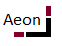
\includegraphics[width=0.2\textwidth]{../Templates/Aeon}\\[1cm] % Include a department/university logo - this will require the graphicx package

	%----------------------------------------------------------------------------------------

	\vfill % Push the date up 1/4 of the remaining page

\end{titlepage}


\section*{\begin{center}Projektidentitet\end{center}}
    \vspace{-2.5em}
    \begin{center}
        \begin{tabular}{|c c c|}
        \hline
        Namn & Roll & E-post \\
        \hline
        Adam Andersson& Teamleader & adam.e.a.andersson@gmail.com\\
        \hline
        Niclas Byrsten & Testansvarig & nicby889@student.liu.se\\
        \hline
        Björn Hvass & Konfigurationsansvarig & bjorn.hvass@gmail.com\\
        \hline
        Henrik Lindström & Utvecklingsledare & henli070@student.liu.se\\
        \hline
        Martin Persson & Arkitekturansvarig & marpe902@liu.student.se\\
        \hline
        Christoffer Sjöbersson & Analysansvarig & chrsj812@liu.student.se\\
        \hline
        Tor Utterborn & Dokument- \& Kvalitetsansvarig & tor.utterborn@gmail.com\\
        \hline
        \end{tabular}
    \end{center}

    \begin{center}
        \small
        \textbf{Kund}\\Region Östergötland, 581 91 Linköping.

        \textbf{Kontaktperson hos kund}\\
        Gunnar Nordqvist, IT-arkitekt, 010-1030698, Gunnar.Nordqvist@regionostergotland.se\\
        Erik Sundvall, Informationsarkitekt, 010-1036252, Erik.Sundvall@regionostergotland.se
    \end{center}

\vspace{9em}



\clearpage
\begin{abstract}
\noindent Under iteration två i kandidatprojektet så har gruppen arbetat med att färdigställa dokument som är till hjälp vid utvecklingsfasen. Kandidatrapporten har även påbörjats och skisser till de individuella bidragen är skrivna.
Slutligen så har gruppen reviderat de tidigare inskickade dokumenten utefter den feedback som de fått av handledaren.
\end{abstract}
\clearpage

\section{Dokumentation}
\label{sec:Dokumentation}
De dokument som har sammanställts under den första iterationen är följande:

\textbf{Kandidatarbete, rapporthalva}\\ En påbörjad kandidatrapport, i denna iteration så har avsnitten introduktion, bakgrund, metodkapitel och resultat avhandlats.

\textbf{Individuellt bidrag}\\
Skisser för de individuella bidragen har skrivits, i denna iteration så har medlemmarna beskrivit det ämne som de vill studera samt hur de kan skaffa material att skriva om.

\textbf{Arkitekturdokument}\\ Arkitekturdokumentet beskriver hur systemet kommer se ut.

\textbf{Testplan}\\
Testplanen fungerar som en grund för hur systemet ska testas, så man kan säkerställa att det är ett stabilt system och så att systemet uppnår kraven som finns.

\textbf{Testrapport}\\
En testrapport för iteration två har framställts. Under denna iteration så har enbart tester med pappersprototyper utförts.

\textbf{Dokumentrevidering} \\
Utefter den feedback som gruppen fick för dokumenten i iteration ett så har dessa reviderats.

\section{Kund}
Under iterationen har gruppen haft ett möte med kund om utseendet på produkten.

Alla medlemmar i gruppen skapade en pappersprototyp gällande hur man tänkt sig att slutprodukten skulle kunna se ut. Gruppen höll sedan ett brainstormmöte där de diskuterade varandras bidrag och man kom fram till tre stycken alternativ som redovisades för kund under ett möte.

\section{Måluppfyllnad}
Vi anser att målen med denna iteration till stor del har uppnåtts. Ett till möte med kund kommer hållas gällande prototyp av produkten, men i övrigt så har gruppen blivit färdiga med de uppgifter som planerats in för denna iteration.

\end{document}
